\documentclass[doc,floatsintext]{apa6}

\usepackage[english]{babel}
\usepackage[utf8x]{inputenc}
\usepackage[natbibapa]{apacite}%For APA referencing
\usepackage{amsfonts}
\usepackage{amsmath}
\usepackage{graphicx}
\usepackage{authblk}
\usepackage{microtype}
\usepackage{amssymb}
\usepackage{soul}
\usepackage[prependcaption,colorinlistoftodos]{todonotes}
\usepackage{amsmath}
\usepackage{algorithm}
\usepackage{algpseudocode}
\graphicspath{{Figures/}}

%For possessive citing
% \def\citeapos#1{\citeauthor{#1}'s (\citeyear{#1})}

% %to do notes jp
% \definecolor{aliceblue}{rgb}{0.94, 0.97, 1.0}
% \newcommand{\jptodo}[2][]{\todo[caption={\textbf{NB}}, size=\scriptsize, color = aliceblue, #1]{#2}~}
% \newcommand{\jptodo}[2][]{\vspace{0.1cm} \hfil \todo[caption={\textbf{JP}}, size=\footnotesize, color = aliceblue, inline, #1]{#2}}


\title{\textbf{Cascades across networks are sufficient for the formation of echo chambers: An agent-based model}}

\shorttitle{Network Cascades and Echo Chambers}

\author[1]{Jan-Philipp Fr{\"a}nken}
\author[2 3]{Toby D. Pilditch}
\affil[1]{Department of Psychology, University of Edinburgh}
\affil[2]{School of Geography and the Environment, University of Oxford}
\affil[3]{Department of Experimental Psychology, University College London}

\affiliation{\mbox{}}


\authornote{Correspondence concerning this article should be addressed to Jan-Philipp Fr{\"a}nken, Department of Psychology, University of Edinburgh, 7 George Square, EH8 9JZ, Scotland. E-mail:
jp.franken@ed.ac.uk.}

\abstract{Investigating how echo chambers emerge in social networks offers an important opportunity for understanding and potentially counteracting the retention of digital misinformation and political polarization. The emergence of echo chambers, which might induce intolerance towards opposing views, mislead public and political discourse (e.g., disbelief in climate change) and retention of misinformation, has previously been attributed to psychological biases (e.g., confirmation bias) and inter-individual differences. Using a Bayesian model of source credibility, we find that echo chambers emerge in networks of homogeneous rational agents, as a function of the networks themselves. Critically, we show that echo chambers emerge prior to repeated interaction, requiring only a single cascade. Overall, these findings suggest that psychological biases, inter-individual differences, or repeated interaction between agents are not necessary for the formation of echo chambers. The limitations of this work, implications for potential interventions, and the value of agent-based modeling for the study of echo chambers and related emergent phenomena are discussed.}

\keywords{social networks; echo chambers; information cascades; agent-based modeling; Bayesian modeling}

\begin{document}
\setlength{\parindent}{2em}
\maketitle

\section{Introduction}

As we navigate social media platforms, we are free to construct our networks according to our individual needs: we choose to be friends with some users while we ignore others, we follow ''Influencers'' that inspire us, and we customize our News Feed to align with our interests. Our access to information is blinkered. Consider for example Facebook: a peer-to-peer system with around 2.45 Billion users, a median of 200 friends per user, and an average connectivity (number of friends per user / total number of users) of less than 0.0000002 \%\footnote{Source: \href{https://www.brandwatch.com/blog/facebook-statistics/}{}.}. Combined with a biased selection of News Feed, Influencers, and friends, such limited access to information has been associated with inaccurate representations of the world, including spreading of misinformation \citep{del2016spreading} and fake news \citep{vosoughi2018spread}. 

Over the past decade, several researchers investigated the spreading and retention of misinformation on social media platforms \citep{starbird2014rumors, bessi2015science, del2016spreading} and its implications for e.g., the polarization of opinions \citep{bessi2016users}. However, the scientific community still lacks precise answers to fundamental questions relating to 1) the prevalence of misinformation and fake news in general and 2) their effects on individuals \citep{lazer2018science}. Consequently, the demand for research investigating how misinformation is spread through social media remains an important topic. Recent work suggesting that misinformation spreads faster than true information on Twitter further emphasizes the relevance of understanding digital misinformation\footnote{Source: http://news.mit.edu/2018/study-twitter-false-news-travels-faster-true-stories-0308.}.

% Summarizing these phenomena under the umbrella term ''digital wildfires'', the World Economic Forum (WEF)\footnote{Source: WEF Global Risks Report 2018} repeatedly declared digital misinformation as an important societal threat. 
In order to address this objective, recent work has investigated the impact of echo chambers on digital misinformation. Echo chambers have been defined as enclosed epistemic systems where like-minded others reinforce their  pre-existing beliefs \citep{madsen2018large}. The enclosing nature of echo chambers has been shown to induce intolerance towards opposing views \citep{takikawa2017political}, and empirical research suggests that echo chambers lead to misleading public and political discourse, such as disbelief in climate change \citep{jasny2015empirical, jasny2019echo}. Extending these empirical findings, extensive quantitative analyses has found a structural effect of echo chambers on the viral spread of misinformation \citep{tornberg2018echo, del2016spreading}. Investigating how echo chambers emerge on social media thus offers an important opportunity for understanding and potentially counteracting the occurrence of digital misinformation. 

\subsubsection{Isolating the causes of echo chambers}
To investigate when and how echo chambers emerge, it is important to isolate their causes. These might be routed in psychological biases: previous analyses of echo chambers and their impact on digital misinformation identified confirmation bias and social influence as key driving factors of echo chamber formation
\citep{del2016spreading}. Similarly, work in statistical physics has shown that confirmation bias induces clustering of like-minded individuals (i.e., echo chambers) and proliferation of opinions \citep{ngampruetikorn2016bias}. Additionally, it has been argued that cognitive differences between individuals might lead to the formation of echo chambers \citep{barkun2013culture}. Together, these findings suggest that psychological variables and cognitive variability among individual agents are necessary requirements for the formation of echo chambers. 

Aiming to clarify the necessity of psychological variables and heterogeneity, recent simulation-based work has investigated echo chamber formation in a population of homogeneous rational (i.e., Bayesian) agents engaging in repeated interaction \citep{madsen2018large, madsen2017growing}. Results provided a formal argument for the inherent susceptibility of social networks towards echo chamber formation despite \emph{absence} of psychological biases (e.g., confirmation bias) and cognitive differences among agents. In other words, the findings of \cite{madsen2018large} suggest that the \textit{structure} of social networks alone is sufficient for the formation of echo chambers. 
% As such, this work showed that previously identified causes of echo chambers, including confirmation bias and cognitive differences among individuals, are not \emph{necessary} for the emergence of echo chambers. 
Importantly, the findings of \citep{madsen2018large, madsen2017growing} are based on repeated interaction between agents. However, work on information cascades has shown that ''single-shot'' cascades result in maladaptive collective outcomes prior to repeated interaction, and despite individually rational agents \citep{bikhchandani1992theory, pilditch2017opinion}. Consequently, a single pass-through of information between generations of agents that update their beliefs sequentially might suffice for the emergence of echo chambers. In other words, the connectivity density of social networks---including lateral transmission of information and limited access to the knowledge of the entire network---might result in echo chamber formation even before repeated interaction.
% The present work is motivated by the structural changes to peer-to-peer systems over the past decades, which have become increasingly centered on online communication using social media, across professional domains \citep{treem2013social}, universities \citep{siddiqui2016social}, and every day life \citep{whiting2013people}. Information transmission through social media platforms differs from classical information systems (e.g., newspapers) where a clear demarcation between content produces and content consumers 

In the present contribution, we aim to extend the reviewed work on echo chambers and digital misinformation in three ways. First, we investigated whether echo chambers emerge as a consequence of social network structure (i.e. connectivity density) in the \emph{absence} of repeated interaction. Specifically, we focused on a single cascade, meaning that all agents updated their beliefs sequentially through a single interaction. Second, building up on previous work by \citep{madsen2017growing, madsen2018large}, we employed an agent-based model in which we isolated structural aspects of a network from psychological variables and inter-individual differences among agents. Therefore, agents in our network were furnished with the same cognitive architecture, forming beliefs normatively through Bayesian updating. Third, we extended the standard Bayesian model used in previous simulations by a more sophisticated model including an analytical cue for the perceived credibility of network inhabitants (see Bayesian source credibility model). Given these advancements, we hope to further clarify the relationship between the various conflated causes of echo chambers and their implications for the retention of digital misinformation. The next section introduces the details of our agent-based model.


\subsection{Agent-based model}
\subsubsection{Conceptual overview}
We reconstructed an idealized social network in which users (i.e., agents) form binary beliefs through a single interaction between generations.
%More specifically, agents 1) payed attention to the beliefs others, 2) updated their prior beliefs based the observed beliefs, and 3) shared their newfangled beliefs with their friends. 
As such, our agent-based model (ABM) captured agents' social environment and temporal dynamics of belief change, which both form necessary requirements for the observation of emergent phenomena such as echo chambers \citep{madsen2019analytic}. Additionally, our ABM accounted for heterogeneity between individual agents (such as different prior beliefs), which is an important general advantage of agent-based simulations \citep{wilensky2015introduction}. The three central components of ABMs (including our model) are agents, patches, and link. Agents are the actors, and in our social network they correspond to individual users. Agents were furnished with cognitive functions and possible behaviours, including attention (detecting public declarations of others), belief revision (updating a prior belief-state based on observing another agent’s belief), and declaration (commit to a belief using a deterministic decision rule). All agents were furnished with the same cognitive functions and possible behaviours. Links represent edges between agents. In the present model, (bidirectional) links were employed to enable signaling of public belief declarations between agents, and thus represent the (social) network connections. Patches are the building blocks of the \(n\)-dimensional environment inhabited by agents. Like agents, patches can change dynamically to model, for example, fluctuations in fish stock at a specific location in space \citep{bailey2019computational}. In the present model, patches were treated as static objects forming a 2-dimensional environment with no further relevance for  simulations.

\subsubsection{Incorporating source credibility}
Expanding the work by \citep{madsen2017growing, madsen2018large}, we included a measure of the credibility of a source (i.e., an agent/social media user) in our simulations. The credibility of a source plays an important role when integrating their beliefs with our own observations and prior expectations \citep{cuddy2011dynamics, fiske2007universal}. Moreover, source credibility plays a critical role in persuasion and argumentation theory, especially in the context of politics \citep{housholder2014facebook, robinson1999measures, cialdini2007influence}, which has become increasingly influenced by online communication systems such as Facebook \citep{bail2016combining}. Both heuristic accounts, such as the heuristic-systematic model (HSM) \citep{chaiken1999heuristic} and dual-process theories, including the influential elaboration-likelihood model (ELM) \citep{petty1986elaboration} have been used to study the influence of credibility on persuasion, showing a positive general impact of credibility on persuasion \citep{chaiken1994heuristic} that has been extended to specific domains such as exercise intentions \citep{jones2003effects}. 

The problem with these classical theories is their qualitative nature: in both HSM and ELM, the credibility of sources is a simple heuristic that does not allow for a quantitative formalization of credibility. This makes weighting the importance of credibility between different contexts difficult, for example, when two receivers vary in terms of their knowledge about the content of a message. Similarly, if two receivers differ with respect to their critical analysis of a source's messages, the importance of credibility should differ, requiring computation of different credibility weights between receivers \citep{madsen2018method}. The Bayesian account, which models credibility as an analytic cue influencing the probability of accepting a message / updating a belief, provides a quantitative framework for evaluating the importance of source credibility during belief revision \citep{harris2009bayesian, oaksford2007bayesian}. Given the importance of source credibility during belief formation, we extended the standard Bayesian framework through a Bayesian source credibility model (BSCM) in our networks of agents. 

% Using a Bayesian framework for modeling the influence of credibility on belief formation allows not only qualitative (directional) predictions, which are available by HSM and ELM, but also a precise quantitative prediction that can be implemented on an algorithmic level. This is essential for the purpose of our work, which furnishes agents with a quantitative cognitive architecture. 

\subsubsection{Bayesian source credibility model}
The standard normative framework for modeling belief updating is given by Bayes' rule, where a prior belief in a hypothesis is represented as subjective probability \(P(h)\) taking values between 0 and 1. Based on observing new data \(d\), the posterior probability of a hypothesis, \(P(h|d)\), is given by the normalized\footnote{normalization is given by the denominator of Equ. 1, which is equal to the total probability of observing data \(d\) for both levels of the hypothesis (\(h\) and \(\neg h\)).} product of the likelihood \(P(d|h)\) and the prior \(P(h)\):

\begin{equation}
    P(h|d) = \frac{P(d|h)P(h)}{\sum_{h'}P(d|h')P(h')}.              
\end{equation}

As in \cite{madsen2017growing, madsen2018large}, we wanted to ensure that individual differences and psychological biases (e.g., confirmation bias) would not conflate with the impact of network structure on the formation of echo chambers. Consequently, all agents were idealized reasoners adhering to the principles of Bayesian updating. To include the credibility of a source, we expanded the basic normative framework using BSCM \citep{harris2016appeal}. BSCM extends Equ. 1 to include the influence of a source's perceived credibility during belief updating. In the BSCM framework, credibility has two components, expertise \(P(e)\) and trustworthiness \(P(t)\) \citep{harris2016appeal}. The perceived expertise \(P(e)\) of a source refers to the probability of the source's communicated belief being correct. The perceived trustworthiness of a communicating agent, \(P(t)\), refers to the communicators intention to tell the truth. In other words, \(P(t)\) is equal to the probability that a communicating agent wants to communicate its true belief, independent of whether the belief is correct or not. \(P(e)\) and \(P(t)\) are both incorporated within the belief revision process in the present agent-based model (see Fig. 1).



\begin{figure}[!t]
\centering
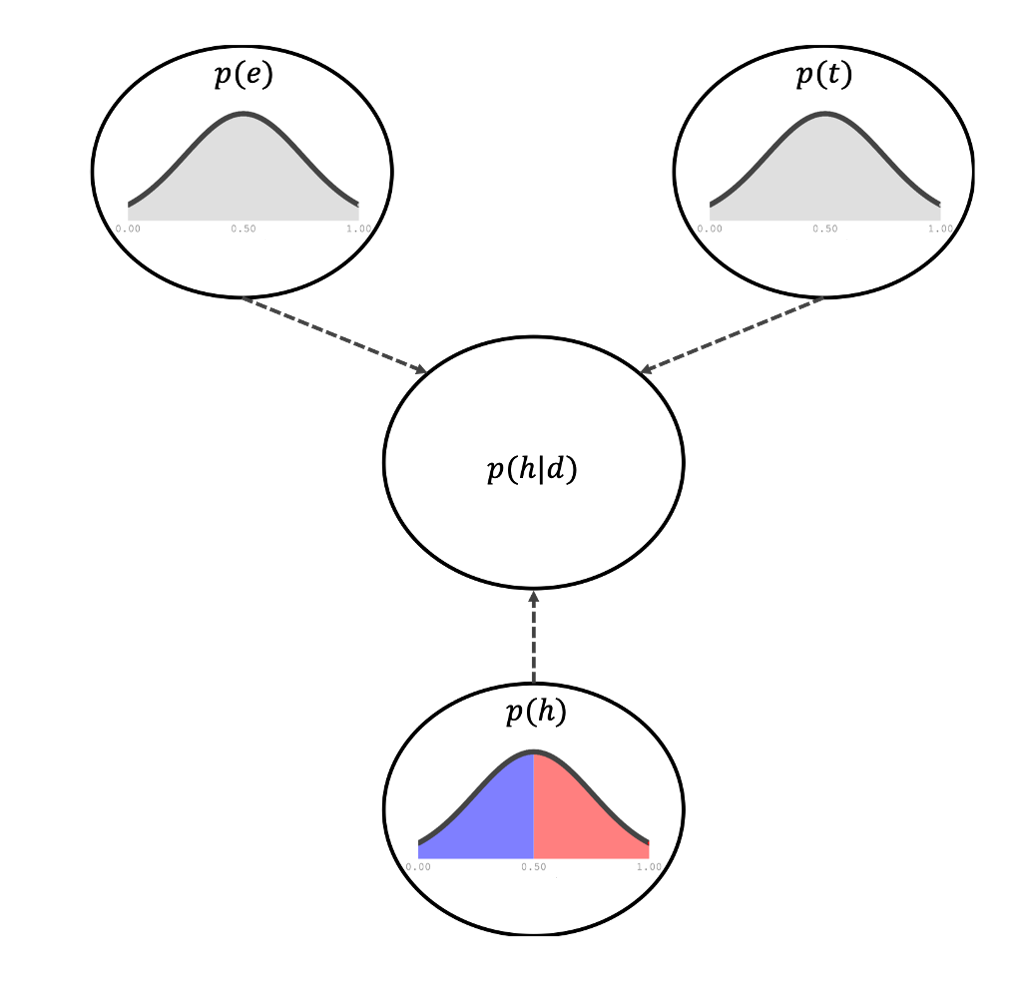
\includegraphics[width=1\columnwidth]{img/bscm_update_2.png}
\caption{Figure shows how a prior belief and the perceived credibility of a source (operationalized via expertise and trustworthiness) interact within the BSCM framework. For the present simulations, agents sampled \(P(h)\), \(P(e)\), and \(P(t)\) estimates from univariate Gaussian distributions (\(\mu\) = 0.50, \(\sigma^2\) = 0.20). Values between 0.00 and 0.50 (blue) =  \(P(\neg h)\); Values between 0.51 and 1.00 (red) =  \(P(h)\). Distributions were truncated (range: [0, 1]).} 
\label{fig:rich_vis}
\end{figure}


In the BSCM framework, the likelihood for an agent that supports a hypothesis  \(P(h)\) is given by

\begin{equation}
    P(d|h) = \sum_{e't'}P(h|e',t')P(e')P(t'). 
\end{equation}

In the same way, the likelihood for an agent that does not support a hypothesis \(P(\neg h)\) corresponds to
   
\begin{equation}
    P(d|\neg h) = \sum_{e't'}P(\neg h|e',t')P(e')P(t'). 
\end{equation}

Table 1 shows the conditional probability table which specified how the different components of the likelihood were computed. Here, expertise, \(\textbf{\emph{e}}\), determines how strongly a communication target is influenced by the expertise of a source. In our simulations, we explored three different parameter settings for expertise  (see Table 2). Similar to an indicator function, \(\textbf{\emph{I}}\) returned 1 for agents having a prior belief \(P(h)\) > 0.5 and -1 for agents having a prior belief \(P(h)\) < 0.5. This procedure ensured that the direction of the influence of expertise matched an agent's prior belief (i.e., towards 1 if \(P(h)\) > 0.5 and towards 0 if  \(P(h)\) < 0.5). \(\tau\) is a constant that accounts for the presence vs. absence of expertise (\(\tau\) = 2 for all simulations).

\begin{table}[!h]
\footnotesize
\begin{center} 
\caption{Conditional probability table.} 
\label{sample-table} 
\vskip 0.10in
\begin{tabular}{c c c c c } 
\hline
 & e,t & \neg e,t & e,\neg t & \neg e,\neg t\\
\hline
h  & \[0.5 + eI_{P(h)>0.5}*\tau \] & \[0.5 + eI_{P(h)>0.5} \] & \[0.5 - eI_{P(h)>0.5}*\tau \] & \[0.5 - eI_{P(h)>0.5}\]\\
\neg h & 1 - (0.5 + eI_{P(h)>0.5}*\tau) & 1 - (0.5 + eI_{P(h)>0.5}) & 1 - (0.5 - eI_{P(h)>0.5}*\tau) & 1 - (0.5 - eI_{P(h)>0.5})\\
\hline
\end{tabular} 
\end{center} 
\end{table}

\subsubsection{Weighting expertise and trustworthiness}
The BSCM architecture provides a general framework for updating one's belief under consideration of a source's credibility. It does not specify how the specific \(e\) and \(t\) should be computed during interaction. Here, each agent is furnished with subjective estimates of \(e\) and \(t\) sampled from a univariate Gaussian. Following observation of a source's belief in a hypothesis, the target agent (receiver) then evaluates the perceived \(e\) and \(t\) of the communicating source as a function of the proportion of agents in the receiver's direct network entertaining the same belief as the source compared to the total number of agents entertaining either the same belief as the source vs. the opposite belief of the source, weighted by the individual expertise and trustworthiness values of agents in the receiver's direct network: 

\begin{equation}
    P(e_{perceived}) = \frac{\sum_{i=1}^{N_h}e_i}{\sum_{i=1}^{N_h}e_i + \sum_{i=1}^{N_{\neg h}}e_i}              
\end{equation}

\begin{equation}
    P(t_{perceived}) = \frac{\sum_{i=1}^{N_h}t_i}{\sum_{i=1}^{N_h}t_i + \sum_{i=1}^{N_{\neg h}}t_i}           
\end{equation}

The perceived credibility weights obtained from Equations 4-5 are then plugged into Equations 2-3 to compute the likelihood of observing a source's belief given the receivers prior belief and the credibility of the source (which is a function of the weighted proportion of agents supporting the same belief as the source compared to the total number of believers in a receiver's network).

\section{Simulations}
Agents were randomly assigned to x-y coordinates in a 2-dimensional space forming \(n\)-links with their nearest neighbors. Proximity was measured in terms of Euclidean distance, which has been used as a proxy for relational proximity in social networks \citep{duggins2017}. Prior to the start of a simulation, each agent sampled their own prior belief \(P(h)\) and subjective \(P(e)\), and \(P(t)\) values from a univariate Gaussian with \(\mu\)=0.5 and \(\sigma^2\)=0.20 (for all three estimates). Thus, \(P(h)\), \(P(e)\), and \(P(t)\) differed heterogeneously within our agent population. Following revision of their prior belief according to BSCM, agents declared for one of the two beliefs based on a deterministic decision rule\footnote{If \(P(h)\) = 0.50, an agent declared either belief with a probability of 50\%.}: 

\[
Belief = \begin{cases}
h \text{ if } P(h|d) > 0.5 \\
\neg h \text{ if } P(h|d) < 0.5 
\end{cases}
\]

The declared belief (i.e. \(h\) or \(\neg h\))  was then made pubic based on the P(Declaration) probability which was manipulated between simulations (see Table 2). For example, a declaration of 1 means all agents made their beliefs public, while 0.1 means that there is a 10\% probability for each agent making their opinion public. In addition to P(Declaration), we varied the interconnectivity between simulations (number of links per agent / total number of agents in the network) from 0.5\% to 50\%. Simulations were initiated through a neutral event node placed in the center of the simulation (i.e. central x-y-coordinate). Neutral in this case means that the first agent sampled randomly from the set of beliefs \{\(h\), \(\neg h\)\} each time it communicated to a target. Due to this stochastic process, on average, half of the \(1\textsuperscript{st}\) generation agents receiving input from the neutral event node should arrive at belief \(h\) while the other half will arrive at belief \(\neg h\) after BSCM integration. The number of agents the neutral event node communicated to was determined by the interconnectivity value. Connectivity values above 50\% were omitted as this would have enabled every other agent to be connected to the neutral event node in the 1st generation, precluding the occurrence of a cascade. Similarly, values below 0.5\% would have resulted in fracturing of the network. 

\begin{table}[!h]
\footnotesize
\begin{center} 
\caption{Manipulated variables.} 
\label{sample-table} 
\vskip 0.10in
\begin{tabular}{c c c} 
\hline
Name & Description & Levels\\
\hline
Interconnectivity (\%) & (Links per Agent / Total Number of Agents) * 100 & 0.5, 1.0, 1.5, ... 50.0\\
Expertise & Manipulate the magnitude of expertise influence & 0.00, 0.10, 0.20\\
P(Declaration) & Probability of making a belief public & 0.10, 0.50, 1.00\\
\hline
\end{tabular} 
\end{center} 
\end{table}

After revising their prior beliefs following the equations outlined in the BSCM section, the first-generation agents (those that received input from the neutral event node) made their beliefs public based on the manipulated P(Declaration) value. Their attentive linked neighbours (i.e., second-generation) then used the communicated opinion of the first-generation agents as input for their own belief revision following the same procedure. Thereafter, the process of transmitting beliefs continued down successive generations until the network was either completely saturated (i.e., all agents committed to a belief) or the number of believers (i.e., \(h\) or \(\neg h\)) did not change for two consecutive time periods. As the goal of the present work was to show that a single pass-through of information (i.e., single interaction) is sufficient for the formation of echo chambers, we did not allow for repeated interaction, meaning that agents were no longer attentive to further information once they declared a belief.

To measure echo chambers effectively across simulations, we were first interested in measuring global proportions of beliefs across the whole network (i.e. the relative number of agents with belief \(h\) compared to agents entertaining belief \(\neg h\)). This measure was necessary to ensure that echo chambers are not a by-product of a dominant network-wide belief. Following checks for possible network-wide belief confounds, our key dependent measure was the average percentage of like-minded neighbours an agent possessed (i.e., the \textit{local} network similarity). This measure corresponded to the average percentage of agents in the target's direct network that shared the same belief as the target. For example, 50\% means that, on average, agents had equal proportions for each belief type in their direct network. We ran each system specification (Interconnectivity (100) x expertise (3) x P(Declaration) (3)) independently 50 times, taking an average set of values for each specification. The total number of agents (n = 1000) was consistent across simulations. Simulations were conducted between two different populations of agents. In the first population, agents computed weighted expertise and trustworthiness values for a source upon detecting their beliefs. In the second population, agents sampled expertise and trustworthiness from a uniform distribution bounded between [0, 1]. This second population functioned as our credibility null hypothesis, as agents sampled stochastic credibility estimates for each source irrespective of the beliefs and credibility values of their network. In other words, these agents were insensitive to beliefs of their social network, considering only their own prior belief and stochastic credibility estimates during revision. 


\section{Results}
Fig. 2 summarizes our central findings. The average proportion of like-minded neighbors in an agent's social network is shown in Fig. 2C (weighted credibility estimates). As evident from the graph, the proportion of like minded neighbors increased as a function of increasing expertise and P(Declaration) and decreasing interconnectivity. Importantly, to fully reduce the formation of echo chambers, the average network member must be connected to around 15-20\% of the network, which is infeasible considering the size of real world social networks which can have several Billion users. Fig. 2D offers a control check for the influence of weighting the credibility values of a source based on an agent's social network. As seen in Fig. 2D, if agents were agnostic of their social network (stochastic sampling of credibility estimates), no echo chambers emerged. The finding in the left panel (P(Declaration) = 10\%) showing a reduced clustering effect for interconnectivity values below 5\% is irrelevant and can be fully attributed to fracturing of the network. Fig. 2A shows that the global proportions of beliefs consistently approximated 50/50 irrespective of varying P(Declaration) or interconnectivity, or expertise. This finding is important, as it shows that clustering of beliefs (Fig. 2C) is not a consequence of a global bias towards either belief. Global belief proportions were similar in the population of agents which was insensitive to their social network during belief updating (Fig 2B). To visualise the above findings, Fig. 3 includes example outcomes of post-cascade belief proportions with 1\% and 5\% interconnectivity. A and C correspond to networks where agents based their credibility estimates on Equations 4-5 (i.e., weighted credibility estimates). B and D are control checks based on stochastic credibility estimates. 


\begin{figure}[!t]
\centering
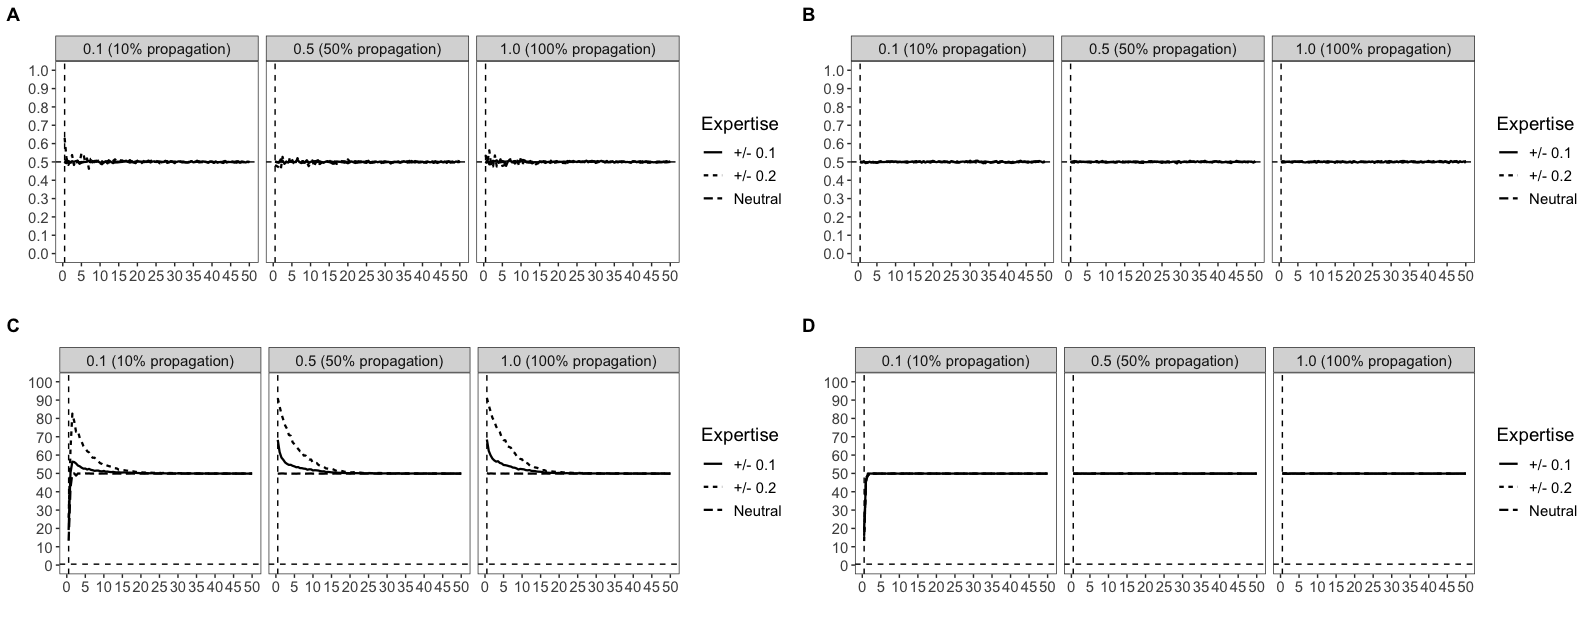
\includegraphics[width=1\columnwidth]{img/results.png}
\caption{Main results. A: global belief proportions, weighted credibility. B: global belief proportions, stochastic credibility. C: average percentage of like-minded neighbors (i.e. echo chambers), weighted credibility. D: average percentage of like-minded neighbors (i.e. echo chambers), stochastic credibility.} 
\label{fig:rich_vis}
\end{figure}


\begin{figure}[!t]
\centering
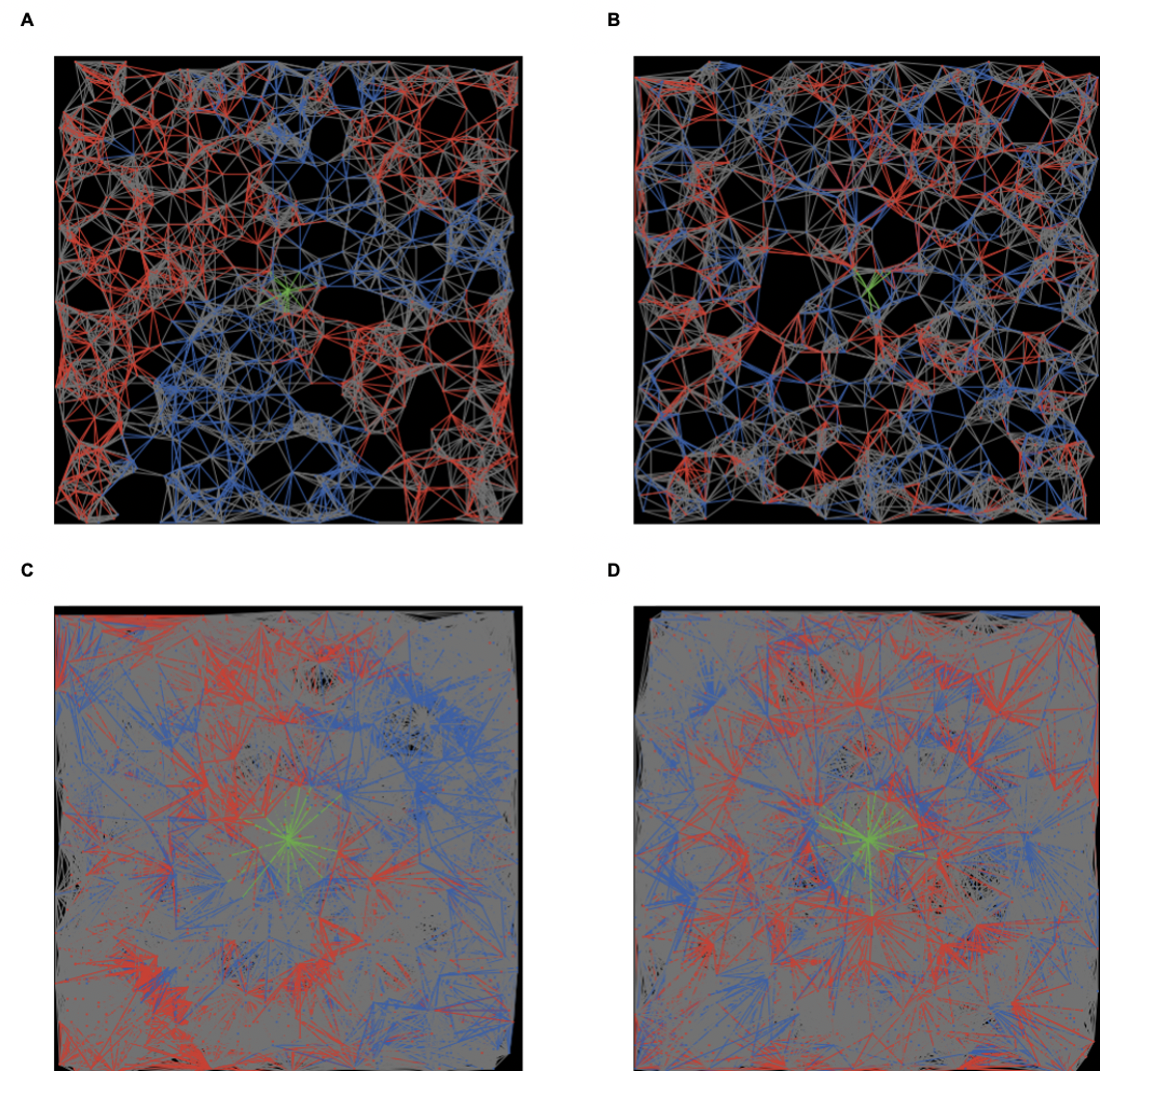
\includegraphics[width=1\columnwidth]{img/example_networks.png}
\caption{Example post-cascade networks. Grey = agents that did not declare a belief; blue = agents believing \(\neg h\); red = agents believing \(h\). Interconnectivity values of upper networks: A (weighted credibility): 1\%; B (stochastic credibility): 1\%. Interconnectivity values of lower networks: C (weighted credibility): 5\%; D (stochastic credibility): 5\%.} 
\label{fig:rich_vis}
\end{figure}


\section{Discussion}
The results of our simulations show that echo chambers emerge as a consequence of interactions between individually rational agents who integrate the beliefs of others with their own prior beliefs in a Bayesian manner. This suggests that previously identified causes of echo chambers, such as confirmation bias and inter-individual differences in terms of the cognitive architecture of agents, are not necessary for the observation of echo chambers. Furthermore, we showed that echo chambers emerge through a single pass-through of information prior to repeated interaction. This finding is critical, as it suggests that repeated interaction, which has been a key component in previous models of echo chambers, might not be required for the formation of echo chambers. On average, each belief was equally represented in our simulations. Thus, our results further show that segregated groups did not evolve as a consequence of a global dominance of a particular belief (see Figs. 2-3). Finally, the comparison of weighted credibility estimates and stochastic credibility estimates revealed that evaluating the credibility of a source based on one's social network was a necessary requirement for echo chamber formation. If agents sampled stochastic credibility values for communicating sources, the network did not show any signs of echo chambers. 

Overall, these findings illustrate that echo chambers, which might induce spreading and retention of misinformation \citep{del2016spreading, tornberg2018echo}, conspiratorial thinking \citep{jasny2015empirical, jasny2019echo}, and political polarization \citep{del2016echo, boutyline2017social, takikawa2017political}, are not necessarily caused by the inhabitants of social networks directly (i.e., individual agents/users). Rather, the \textit{structure} of social networks, and notably the constraining lateral (i.e., peer-to-peer) transmission of information can be sufficient for echo chamber formation.
The degree of making opinions public (P(Declaration)) did affect echo chamber formation only if it was so low that it effectively fractured the functional message passing around the network. Additionally, the magnitude of perceived expertise modulated the influence of credibility, resulting in increased echo chamber effects for higher levels of expertise. This suggests that selecting one's network peers based on friendship might exacerbate the formation of echo chambers. Given that the present simulations included rational Bayesian agents, it is further expected that incorporation of additional psychological variables, such as confirmation bias \citep{del2016spreading, ngampruetikorn2016bias}, might intensify the strength and persistence of echo chambers \citep{pilditch2017opinion}.

More generally, our results show that agent-based models, which enable capturing of dynamic interactions between individuals, provide a valuable opportunity for studying the formation of emergent phenomena such as echo chambers. This is in line with a growing body of literature employing agent-based models to investigate several related phenomena, including opinion polarization \citep{duggins2017}, identity search \citep{watts2002identity}, disbelief in climate change \citep{lewandowsky2019influence} and micro-targeting \citep{madsen2018method}. Given the potential of agent-based models for studying echo chambers and related emergent phenomena, it is important that further work develops interventions which might reduce the occurrence of opinion segregation. Such interventions might extend previous work suggesting that ''educational broadcasts'' across a network of idealized Bayesian agents (similar to the present model) reduce echo chamber formation \citep{madsen2018large}.

In our simulations, agents updated their beliefs sequentially based on the declarations of previous generations. Related theoretical work on information cascades has illustrated that sequential updating processes, where people learn from the beliefs and behaviours of others, can result in erroneous collective outcomes \citep{bikhchandani1992theory}. Critically, this work has shown that erroneous collective behaviours emerged regardless of the fact that people integrated beliefs of others in individually rational ways. However, recent empirical studies demonstrated that people are sensitive to statistical dependencies in social learning. Specifically, across both abstract (e.g., estimating the number marbles in an urn; see \citet{whalen2018sensitivity}) and more applied tasks (e.g., rating the suitability of a political candidate for public office), it has been shown that people differentiate between the evidential signal of independent beliefs and dependent beliefs that were formed sequentially. As a result, given that the beliefs of others were formed sequentially, people updated their prior beliefs to a smaller extent. \cite{whalen2018sensitivity} interpreted this finding as a potential way of counteracting the formation of information cascades, which have been shown to induce convergence towards like-minded clusters \citep{bikhchandani1998learning}. Given these findings, an important step for future research involves testing the robustness of echo chambers between varying levels of belief dependencies in a network. Here, empirical findings by \citep{whalen2018sensitivity} and (...) might be used as input validation for simulation, enabling agents to differentiate between independent and sequentially updated beliefs. 

In summary, while the study of echo chambers does by no means exhaustively addresses the issue of digital misinformation, it provides an important contribution to our understanding of how people settle on beliefs in social networks. Here, we showed that echo chambers emerge as a consequence of social network structure, including limited access to information (i.e., local connectivity) and lateral transmission between peers. This suggests that social networks themselves can be argued to be causally sufficient for echo chamber formation, while previously conflated causes such as psychological biases, inter-individual differences, and repeated interaction, might not be necessary. Rather, such inter-individual differences and psychological variables, including confirmation bias, are expected to exacerbate the formation of echo chambers \citep{pilditch2017opinion}. Finally, by showing that the computations involved in evaluating the credibility of a source play a key role in the formation of echo chambers, our findings might provide important insights for improving the architecture of social networks in a way to be more robust towards echo chamber formation.


\section{Methods}

\subsubsection{Agent-based Simulations}
The presented agent-based model was implemented in NetLogo version 6.0.4 \citep{wilensky1999netlogo}. All simulations were performed in R using the package {\tt RNetLogo()} \citep{thiele2014r}. The full model including all technical details has been uploaded to Github and can be found via \href{}{ link}. Here we outline the three basic steps involved in our model. 

Algorithm 1 shows the setup procedure of the network.


\begin{algorithm}[H]
\caption{Setup Network}\label{setup}
\begin{algorithmic}[1]
  \Procedure{Place agents}{}
    \State Create $N$ agents
    \For{$i=1$ to $N$}
        \State set i position random x-y coordinate
     \EndFor
  \EndProcedure
  \Procedure{Setup priors and Links}{}
    \For{$i=1$ to $N$}
      \State $P(h)[i]\gets x$\thicksim$N(\mu, \sigma^2)$ 
      \State $P(e)[i]\gets x$\thicksim$N(\mu, \sigma^2)$
      \State $P(t)[i]\gets x$\thicksim$N(\mu, \sigma^2)$
      \State create links with $n$ nearest neighbors \Comment{based on Euclidean distance}
     \EndFor
  \EndProcedure
\end{algorithmic}
\end{algorithm}

Algorithm 2 shows the basic steps involved in a single instance of belief updating (i.e., from one generation to the the next). Here, source refers to an agent from the previous generation that already publicly declared a belief (i.e., \(h\) or \(\neg h\)).

\begin{algorithm}[H]
\caption{Updating beliefs}\label{update}
\begin{algorithmic}[1]
  \Procedure{Source selects communication target}{}
    \If{matchCounter $\leq$ 1}
        \For{$i=1$ to $n_{source}$}\Comment{n = source's connections}
            \If{i = neutral}\Comment{check if agent did not already declare a belief}
             \State belief[i] = BSCM(source, n[i])\Comment{n = target's connections}
              \If{random(0.01,1.00) > P(Declaration)}
               \State propagate belief to next generation
              \EndIf
             \EndIf
        \EndFor
    \EndIf
  \EndProcedure
\end{algorithmic}
\end{algorithm}

Algorithm 3 illustrates how the {\tt matchCounter} variable shown above was updated. If there was no change in overall proportions of beliefs for two consecutive time periods (i.e., the network was either saturated or fractured), simulations stopped.

\begin{algorithm}[H]
\caption{Proceed to next generation}\label{proceed}
\begin{algorithmic}[1]
  \Procedure{Check if network is saturated or fractured}{}
    \State matchCounter = 0 \Comment{counts how often no change occurred between generations}
    \State Count_{\(h\)} = 0
    \State Count_{\(\neg h\)} = 0
    \For{$i=1$ to $N$}\Comment{N = all agents}
        \If{belief[i] = \(h\)}
            \State Count_{\(h\)} = Count_{\(h\)} + 1
        \EndIf
        \If{belief[i] = \(\neg h\)}
            \State Count_{\(\neg h\)} = Count_{\(\ \)} + 1
        \EndIf
    \EndFor
    \If{Count_{\(h\)} = Count_{\(\neg h\)}}
        \State matchCounter = matchCounter + 1
    \EndIf
  \EndProcedure
\end{algorithmic}
\end{algorithm}

\newpage

\bibliographystyle{apacite}
\bibliography{refs}


\end{document}